\documentclass[a4paper,UKenglish]{lipics-v2018}

\usepackage{microtype}
\usepackage{proof}
\usepackage[dvipsnames]{xcolor}
\usepackage{amsmath}
\usepackage{stmaryrd}

\bibliographystyle{plainurl}

% Author macros::begin %%%%%%%%%%%%%%%%%%%%%%%%%%%%%%%%%%%%%%%%%%%%%%%%
\title{A Syntax for Higher Inductive-Inductive Types}
%\titlerunning{} %optional, in case that the title is too long; the running title should fit into the top page column

%% Please provide for each author the \author and \affil macro, even when authors have the same affiliation, i.e. for each author there needs to be the  \author and \affil macros
\author{Ambrus Kaposi}{Faculty of Informatics, E{\"o}tv{\"o}s Lor{\'a}nd University, P{\'a}zm{\'a}ny P{\'e}ter s{\'e}t{\'a}ny 1/C, 1117 Budapest, Hungary}{akaposi@inf.elte.hu}{https://orcid.org/0000-0001-9897-8936}{}
\author{András Kovács}{Faculty of Informatics, E{\"o}tv{\"o}s Lor{\'a}nd University, P{\'a}zm{\'a}ny P{\'e}ter s{\'e}t{\'a}ny 1/C, 1117 Budapest, Hungary}{kovacsandras@inf.elte.hu}{https://orcid.org/0000-0002-6375-9781}{}
\authorrunning{A. Kaposi and A. Kovács} %mandatory. First: Use abbreviated first/middle names. Second (only in severe cases): Use first author plus 'et. al.'

\Copyright{Ambrus Kaposi and András Kovács}%mandatory, please use full first names. LIPIcs license is "CC-BY";  http://creativecommons.org/licenses/by/3.0/

\subjclass{Theory of computation $\rightarrow$ Type theory}
\keywords{homotopy type theory, inductive-inductive types, higher inductive types, quotient inductive types, logical relations}% mandatory: Please provide 1-5 keywords

\funding{This work was supported by the European Union, co-financed by
  the European Social Fund (EFOP-3.6.3-VEKOP-16-2017-00002), USAF
  grant FA9550-16-1-0029, and by COST Action EUTypes CA15123.}

\acknowledgements{The authors thank Thorsten Altenkirch, Simon
  Boulier, Paolo Capriotti, Péter Diviánszky, Gábor Lehel and Nicolas
  Tabareau for discussions related to this paper and the anonymous
  reviewers for their helpful comments and suggestions. We thank
  Balázs Kőműves for the idea of using a Tarski universe instead of a
  Russell universe in the theory of codes.}

% Author macros::end %%%%%%%%%%%%%%%%%%%%%%%%%%%%%%%%%%%%%%%%%%%%%%%%%

%Editor-only macros:: begin (do not touch as author)%%%%%%%%%%%%%%%%%%%%%%%%%%%%%%%%%%
\EventEditors{H\'{e}l\`{e}ne Kirchner}
\EventNoEds{1}
\EventLongTitle{3rd International Conference on Formal Structures for Computation and Deduction (FSCD 2018)}
\EventShortTitle{FSCD 2018}
\EventAcronym{FSCD}
\EventYear{2018}
\EventDate{July 9--12, 2018}
\EventLocation{Oxford, UK}
\EventLogo{}
\SeriesVolume{108}
\ArticleNo{20}
% Editor-only macros::end %%%%%%%%%%%%%%%%%%%%%%%%%%%%%%%%%%%%%%%%%%%%%%%

%=====================================================================

%% setting \sqcdot as HoTT-book-style transitivity
\makeatletter
\DeclareRobustCommand{\sqcdot}{\mathbin{\mathpalette\morphic@sqcdot\relax}}
\newcommand{\morphic@sqcdot}[2]{%
  \sbox\z@{$\m@th#1\centerdot$}%
  \ht\z@=.33333\ht\z@
  \vcenter{\box\z@}%
}
\makeatother

\newcommand{\U}{\mathsf{U}}
\newcommand{\El}{\mathsf{El}}
\newcommand{\REN}{\mathsf{REN}}
\newcommand{\op}{\mathsf{op}}
\newcommand{\ra}{\rightarrow}
\newcommand{\Ra}{\Rightarrow}
\newcommand{\Set}{\mathsf{Set}}
\newcommand{\PSh}{\mathsf{PSh}}
\newcommand{\FamPSh}{\mathsf{FamPSh}}
\renewcommand{\ll}{\llbracket}
\providecommand{\rr}{\rrbracket}
\newcommand{\Con}{\mathsf{Con}}
\newcommand{\Ty}{\mathsf{Ty}}
\newcommand{\Tm}{\mathsf{Tm}}
\newcommand{\Tms}{\mathsf{Tms}}
\newcommand{\R}{\mathsf{R}}
\newcommand{\TM}{\mathsf{TM}}
\newcommand{\NE}{\mathsf{NE}}
\newcommand{\NF}{\mathsf{NF}}
\newcommand{\p}{\mathsf{p}}
\newcommand{\q}{\mathsf{q}}
\renewcommand{\u}{\mathsf{u}}
\renewcommand{\ne}{\mathsf{ne}}
\newcommand{\nf}{\mathsf{nf}}
\newcommand{\lQ}{\mathsf{lQ}}
\newcommand{\lU}{\mathsf{lU}}
\renewcommand{\lq}{\mathsf{lq}}
\newcommand{\lu}{\mathsf{lu}}
\newcommand{\cul}{\ulcorner}
\newcommand{\cur}{\urcorner}
\newcommand{\norm}{\mathsf{norm}}
\newcommand{\Nf}{\mathsf{Nf}}
\newcommand{\Ne}{\mathsf{Ne}}
\newcommand{\Nfs}{\mathsf{Nfs}}
\newcommand{\Nes}{\mathsf{Nes}}
\newcommand{\ID}{\mathsf{ID}}
\newcommand{\id}{\mathsf{id}}
\newcommand{\nat}{\,\dot{\rightarrow}\,}
%\newcommand{\nat}{\overset{\mathsf{n}}{\ra}} % this is how we denote it in the formalisation
\newcommand{\Nat}{\mathsf{Nat}}
\renewcommand{\S}{\overset{\mathsf{s}}{\ra}} % we have it with uppercase S in the formalisation
\newcommand{\blank}{\mathord{\hspace{1pt}\text{--}\hspace{1pt}}} %from the book
%\newcommand{\blank}{\!{-}\!}
\newcommand{\lam}{\mathsf{lam}}
\newcommand{\app}{\mathsf{app}}
\newcommand{\tr}[2]{\ensuremath{{}_{#1 *}\mathopen{}{#2}\mathclose{}}}
\newcommand{\C}{\mathsf{C}}
\newcommand{\Code}{\mathsf{Code}}
\newcommand{\M}{\mathsf{M}}
% from the book
%\newcommand{\M}{{\scalebox{0.6}{$\mathsf{M}$}}}
%% \newcommand{\C}{\mathcal{C}}
\newcommand{\data}{\mathsf{data}}
\newcommand{\ind}{\hspace{1em}}
\newcommand{\idP}{\mathsf{idP}}
\newcommand{\compP}{\mathsf{compP}}
\newcommand{\idF}{\mathsf{idF}}
\newcommand{\compF}{\mathsf{compF}}
\newcommand{\proj}{\mathsf{proj}}
\newcommand{\ExpPSh}{\mathsf{ExpPSh}}
\newcommand{\map}{\mathsf{map}}
\newcommand{\Var}{\mathsf{Var}}
\newcommand{\Vars}{\mathsf{Vars}}
\newcommand{\wk}{\mathsf{wk}}
\newcommand{\neuU}{\mathsf{neuU}}
\newcommand{\neuEl}{\mathsf{neuEl}}
\newcommand{\var}{\mathsf{var}}
\newcommand{\natn}{\mathsf{natn}}
\newcommand{\natS}{\mathsf{natS}}
\newcommand{\LET}{\mathsf{let}}
\newcommand{\IN}{\mathsf{in}}
\newcommand{\refl}{\mathsf{refl}}
\newcommand{\trans}{\mathbin{\raisebox{0.2ex}{$\displaystyle\centerdot$}}}
\newcommand{\zero}{\mathsf{zero}}
\newcommand{\suc}{\mathsf{suc}}
\newcommand{\N}{\mathbb{N}}

\newcommand\arcfrombottom{
  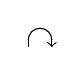
\begin{tikzpicture}[scale=0.03em]
    \draw (0,0) arc (0:180:0.5);
    \draw (0,0) edge[->] (0,-0.3);
    \draw (-1,0) edge (-1,-0.3);
  \end{tikzpicture}
}
\newcommand\arcfromtop{
  
\begin{tikzpicture}[scale=0.03em]
    \draw (0,0) arc (180:360:0.5);
    \draw (0,0) edge[->] (0,0.3);
    \draw (1,0) edge (1,0.3);
  \end{tikzpicture}
}

\newcommand{\Elim}{\mathsf{Elim}}
\newcommand{\elim}{\mathsf{elim}}
\newcommand{\Rec}{\mathsf{Rec}}
\newcommand{\record}{\mathsf{record}}
\newcommand{\funext}{\mathsf{funext}} \newcommand{\Q}{\mathsf{Q}}
\newcommand{\T}{\mathsf{T}} \newcommand{\leaf}{\mathsf{leaf}}
\newcommand{\node}{\mathsf{node}} \newcommand{\perm}{\mathsf{perm}}
\newcommand{\coe}{\mathsf{coe}} \newcommand{\vz}{\mathsf{vz}}
\newcommand{\vs}{\mathsf{vs}} \newcommand{\untr}{\mathsf{untr}}
\newcommand{\from}{\mathsf{from}}
\newcommand{\fromeq}{{\mathsf{from}\hspace{-0.3em}\equiv}}
\newcommand{\fromsimeq}{{\mathsf{from}\hspace{-0.3em}\simeq}}
\newcommand{\Model}{\mathsf{Model}}
\newcommand{\DModel}{\mathsf{DModel}}
\newcommand{\module}{\mathsf{module}}
\newcommand{\open}{\mathsf{open}}
\renewcommand{\P}{\mathsf{P}} \newcommand{\Bool}{\mathsf{Bool}}
\newcommand{\true}{\mathsf{true}} \newcommand{\false}{\mathsf{false}}
\renewcommand{\not}{\mathsf{not}} \newcommand{\0}{\mathsf{0}}
\newcommand{\1}{\mathsf{1}} \renewcommand{\Pr}{\mathsf{Pr}}
\newcommand{\PrNat}{\mathsf{PrNat}} \newcommand{\J}{\mathsf{J}}
\newcommand{\wkV}{\mathsf{wkV}} \renewcommand{\r}[1]{{\P_{#1}}}
\newcommand{\stab}{\mathsf{stab}} \newcommand{\NTy}{\mathsf{NTy}}
\newcommand{\isDec}{\mathsf{isDec}} \newcommand{\dec}{\mathsf{dec}}
\newcommand{\yes}{\mathsf{yes}} \newcommand{\no}{\mathsf{no}}
\newcommand{\case}{\mathsf{case}} \newcommand{\inj}{\mathsf{inj}}
\newcommand{\K}{\mathsf{K}} \newcommand{\lb}{\langle}
\newcommand{\rb}{\rangle} \newcommand{\Decl}{\mathsf{Decl}}
\newcommand{\Core}{\mathsf{Core}} \newcommand{\IND}{\mathsf{ind}}
\newcommand{\Id}{\mathsf{Id}} \newcommand{\Base}{\mathsf{Base}}
\newcommand{\Setoid}{\mathsf{Setoid}}
\newcommand{\FamSetoid}{\mathsf{FamSetoid}}
\newcommand{\prop}{\mathsf{prop}} \newcommand{\resp}{\mathsf{resp}}
\newcommand{\transport}{\mathsf{transport}}
\newcommand{\I}{\mathsf{I}} \newcommand{\E}{\mathsf{E}}
\newcommand{\transp}{\mathsf{transp}}
\newcommand{\Transp}{\mathsf{Transp}}
\newcommand{\W}{\mathsf{W}}
\newcommand{\Fin}{\mathsf{Fin}} \newcommand{\fzero}{\mathsf{fzero}}
\newcommand{\fsuc}{\mathsf{fsuc}}
\newcommand{\inv}{\mathsf{inv}}
\newcommand{\con}{\mathsf{con}}
\newcommand{\LEFT}{\mathsf{left}}
\newcommand{\RIGHT}{\mathsf{right}}
\newcommand{\seg}{\mathsf{seg}}
\newcommand{\Int}{\mathsf{Int}}
\renewcommand{\in}{\mathbin{\hat:}}
\renewcommand{\hat}[1]{{\color{BrickRed}{#1}}}
\newcommand{\vdashh}{\mathbin{\hat\vdash}}
\newcommand{\rah}{\mathbin{\hat\ra}}
\newcommand{\commah}{\hat,\,}
\newcommand{\timesh}{\mathbin{\hat\times}}
\newcommand{\eqh}{\mathbin{\hat=}}
\newcommand{\TR}{\hat{\mathsf{tr}}}
\newcommand{\ap}{\hat{\mathsf{ap}}}
\newcommand{\apd}{\hat{\mathsf{apd}}}
\renewcommand{\tt}{\hat{\mathsf{tt}}}
\newcommand{\Tel}{\hat{\mathsf{Tel}}}
\newcommand{\Type}{\hat{\mathsf{Type}}}
\newcommand{\emptytel}{\hat{\epsilon}}
\newcommand{\telext}{\mathbin{\hat{\lhd}}}
\newcommand{\ltel}{\hat{\ll}}
\newcommand{\rtel}{\hat{\rr}}
\newcommand\pp{\ensuremath{\hat{\mathbin{+\mkern-10mu+}}}}
\newcommand{\semicol}{\hat;\,}
\newcommand{\targetass}{\hat{\Gamma}\semicol}
%\newcommand{\targetass}{;}

%=====================================================================

\begin{document}

\maketitle

%=====================================================================

\begin{abstract}
Higher inductive-inductive types (HIITs) generalise inductive types of
dependent type theories in two directions. On the one hand they allow
the simultaneous definition of multiple sorts that can be indexed over
each other. On the other hand they support equality constructors, thus
generalising higher inductive types of homotopy type theory. Examples
that make use of both features are the Cauchy reals and the well-typed
syntax of type theory where conversion rules are given as equality
constructors. In this paper we propose a general definition of HIITs
using a domain-specific type theory. A context in this small type
theory encodes a HIIT by listing the type formation rules and
constructors. The type of the elimination principle and its
$\beta$-rules are computed from the context using a variant of the
syntactic logical relation translation. We show that for indexed
W-types and various examples of HIITs the computed elimination
principles are the expected ones. Showing that the thus specified
HIITs exist is left as future work. The type theory specifying HIITs
was formalised in Agda together with the syntactic translations. A
Haskell implementation converts the types of sorts and constructors
into valid Agda code which postulates the elimination principles and
computation rules.
\end{abstract}

%=====================================================================

\section{Introduction}
\label{sec:intro}

Many dependent type theories support some form of inductive types. An
inductive type is given by its constructors, along with an elimination
principle which expresses that all inhabitants are constructed using
finitely many applications of the constructors.

For example, the inductive type of natural numbers $\Nat$ is given by
the constructors $\zero:\Nat$ and $\suc:\Nat \ra \Nat$. The
eliminator corresponds to the usual notion of mathematical induction:
\[
  \Elim\Nat:(P:\Nat \ra \mathsf{Type})(pz: P\,\zero)\big(ps:(n:\Nat)\ra P\,n\ra P\,(\suc\,n)\big)(n:\Nat)\ra P\,n
\]
$P$ is a family of types over natural numbers, which is called the
\emph{motive} of the eliminator. It can be viewed as a proof-relevant
predicate on $\Nat$. The arguments $pz$ and $ps$ are called the
\emph{methods} of the eliminator. The \emph{target} of the eliminator
is $n$ and given methods for each constructor, the eliminator provides
a witness of $P\,n$. Thus, if $P$ holds for $\zero$ and $\suc$
preserves $P$, then $P$ holds for all natural numbers. The behaviour
of the eliminator is described by a \emph{computation-rule}
($\beta$-rule) for each constructor:
\begin{alignat*}{5}
  & \Elim\Nat\,P\,pz\,ps\,\zero && \equiv pz \\
  & \Elim\Nat\,P\,pz\,ps\,(\suc\,n) && \equiv ps\,n\,(\Elim\Nat\,P\,pz\,ps\,n)
\end{alignat*}
These express that the eliminator applied to a constructor expression
reduces to an application of the corresponding induction method. From
an operational point of view, $\Elim\Nat$ replaces all the $\zero$ and
$\suc$ constructors with the given induction methods.

% A special case of the eliminator is the recursor (non-dependent
% eliminator) which allows the definition of a non-dependent function
% from the inductive type, for $\Nat$ it has the following type.
% \[
% \Rec\Nat : \forall(A:\mathsf{Type}).A \ra (A \ra A) \ra \Nat \ra A
% \]
% The eliminator can be derived from the recursor and a uniqueness
% principle.

Dependent families of types can be defined in a similar way, for
example vectors of $A$-elements $\mathsf{Vec}_A: \Nat \ra \mathsf{Type}$ which
are indexed by their length. Another generalisation of inductive types
are mutual inductive types. However, these can be reduced to indexed
families where indices classify constructors for each mutual type.
Inductive-inductive types \cite{forsberg-phd} are mutual definitions
where this reduction does not work: here a type is defined together
with a family indexed over it. An example is the following fragment of
the well-typed syntax of type theory where the second sort $\Ty$ is
indexed over the first sort $\Con$, but constructors of $\Con$ also
refer to $\Ty$:
\begin{alignat*}{3}
  & \Con && : \mathsf{Type} && \text{sort of contexts} \\
  & \Ty  && : \Con \ra \mathsf{Type} && \text{sort of types given a context} \\
  & \bullet && : \Con && \text{constructor for the empty context} \\
  & \blank\rhd\blank && : (\Gamma:\Con)\ra\Ty\,\Gamma\ra\Con && \text{constructor for context extension} \\
  & \U && : (\Gamma:\Con)\ra\Ty\,\Gamma && \text{constructor for a base type} \\
  & \Pi && : (\Gamma:\Con)(A:\Ty\,\Gamma)\ra\Ty\,(\Gamma\rhd A)\ra\Ty\,\Gamma \hspace{1em} && \text{constructor for dependent functions}
\end{alignat*}
There are two eliminators for this type: one for $\Con$ and one for
$\Ty$. Both take the same arguments: two motives ($P:\Con\ra\mathsf{Type}$ and
$Q:(\Gamma:\Con)\ra P\,\Gamma\ra\Ty\,\Gamma\ra\mathsf{Type}$) and four methods
(one for each constructor, we don't list these).
\begin{alignat*}{6}
  & \Elim\Con && : (P:\dots)(Q:\dots)\ra\dots\ra(\Gamma:\Con) && \ra P\,\Gamma \\
  & \Elim\Ty  && : (P:\dots)(Q:\dots)\ra\dots\ra(A:\Ty\,\Gamma) && \ra Q\,\Gamma\,(\Elim\Con\,\Gamma)\,A
\end{alignat*}
Note that the type of $\Elim\Ty$ refers to $\Elim\Con$, which is why
this elimination principle is called recursive-recursive (analogously
to the phrase ``inductive-inductive'').

Higher inductive types (HITs, \cite[Chapter 6]{HoTTbook}) generalise
inductive types in a different way: they allow constructors expressing
equalities of elements of the type being defined. This enables, among
others, the definition of types quotiented by a relation. For example,
the type of integers $\Int$ can be given by a constructor
$\mathsf{pair}:\Nat\ra\Nat\ra\Int$ and an equality constructor
$\mathsf{eq}:(a\,b\,c\,d:\Nat)\ra a+d=_\Nat b+c\ra
\mathsf{pair}\,a\,b=_{\Int}\mathsf{pair}\,c\,d$ targetting an equality
of $\Int$. The eliminator for $\Int$ expects a motive
$P:\Int\ra\mathsf{Type}$, a method for the $\mathsf{pair}$ constructor
$p:(a\,b:\Nat)\ra P\,(\mathsf{pair}\,a\,b)$ and a method for the
equality constructor $\mathsf{path}$. This method is a proof that
given $e:a+d=_\Nat b+c$, $p\,a\,b$ is equal to $p\,c\,d$ (the types of
which are equal by $e$). Thus the method for the equality constructor
ensures that all functions defined from the quotiented type respect
the relation. Since the integers are supposed to be a set (which
means that any two equalities between the same two integers are
equal), we would need an additional higher equality constructor
$\mathsf{trunc}:(x\,y:\Int)\ra(p\,q:x=_\Int y)\ra p=_{x=_\Int y} q$.
HITs allow equality constructors at any level. With the view of types
as spaces in mind, point constructors add points to the space,
equality constructors add paths and higher constructors add homotopies
between paths.

Not all constructor expressions make sense. For example \cite[Example
  6.13.1]{HoTTbook}, given an $f:(X:\mathsf{Type})\ra X\ra X$, suppose that an
inductive type $\mathsf{Ival}$ is generated by the point constructors
$\mathsf{a}:\mathsf{Ival}$, $\mathsf{b}:\mathsf{Ival}$ and a path
constructor $\sigma:f\,\mathsf{Ival}\,\mathsf{a}
=_{\mathsf{Ival}}f\,\mathsf{Ival}\,\mathsf{b}$. The eliminator for this type
should take a motive $P:\mathsf{Ival}\ra\mathsf{Type}$, two methods $p_a :
P\,\mathsf{a}$ and $p_b : P\,\mathsf{b}$, and a path connecting
elements of $P\,(f\,\mathsf{Ival}\,\mathsf{a})$ and
$P\,(f\,\mathsf{Ival}\,\mathsf{b})$. However it is not clear what these
elements should be: we only have elements $p_a:P\,\mathsf{a}$ and
$p_b:P\,\mathsf{b}$, and there is no way in general to transform these
to have types $P\,(f\,\mathsf{Ival}\,\mathsf{a})$ and
$P\,(f\,\mathsf{Ival}\,\mathsf{b})$.

Another invalid example is an inductive type $\mathsf{Neg}$ with a
constructor $\con:(\mathsf{Neg} \ra \bot) \ra \mathsf{Neg}$ where $\bot$
is the empty type. An eliminator for this type should (at least) yield
a projection function $\proj: \mathsf{Neg} \ra (\mathsf{Neg} \ra
\bot)$. Given this, we can define $u :\equiv \con\,(\lambda x
. \proj\, x\,x):\mathsf{Neg}$ and then derive $\bot$ by
$\proj\,u\,u$. The existence of $\mathsf{Neg}$ would make the type
theory inconsistent. A common restriction to avoid such situations is
\emph{strict positivity}. It means that the type being defined cannot
occur on the left hand side of a function arrow in a parameter of a
constructor. This excludes the above constructor $\con$.

In this paper we propose a general syntax for higher
inductive-inductive types (HIITs) which includes the above positive
examples and excludes the negative ones. Our syntax for HIITs allows
any number of inductive-inductive sorts, possibly infinitary higher
constructors of any dimension and restricts constructors to strictly
positive ones. It also allows free usage of $\J$ and $\refl$ in HIIT
specifications.  We also show how to derive the types of the
eliminators and computation rules from the type formation rules and
constructors.

The core idea is to represent HIIT specifications as contexts in a
domain-specific type theory which we call the \emph{theory of
  codes}. A context in this theory can be seen as a \emph{code} for a
HIIT, similarly to how a container \cite{abbot05containers} can be
seen as a code for a simple inductive type. Type formers in the theory
of codes are restricted in order to enforce strict positivity. For
example, natural numbers are defined as the three-element context
\[
  Nat:\U,\,\,\, zero:\underline{Nat},\,\,\, suc : Nat \ra \underline{Nat}
\]
where $Nat$, $zero$ and $suc$ are simply variable names, and underlining
denotes $\El$ (decoding) for the Tarski-style universe $\U$.

We use a variant of Bernardy et al.'s logical predicate translation
\cite{bernardy2010parametricity} to derive the types of motives and
methods, and a logical relation translation to derive the types of the
eliminators and computation rules. The target of these translations is
a type theory with a predicative hierarchy of Russell-style universes
closed under $\Pi$, $\Sigma$, the equality (identity) type
$\blank=\blank$ and the unit type $\top$. The source type theory is
the target type theory extended with rules for the theory of codes.

To our knowledge, this is the first proposal for a definition of
HIITs. Proving the existence of the HIITs thus specified is left as
future work.

\subsection{Overview of the paper}

We start by describing the target type theory in Section
\ref{sec:target}. In Section \ref{sec:source}, we define the source
type theory. The source type theory is the target theory extended with
the theory of codes, i.e.\ the rules to describe HIITs. We also
provide several examples of HIIT definitions. In Section
\ref{sec:translation} we define three syntactic translations from the
source to the target theory, each depending on the previous one:
first, we compute the types of type formation rules and constructors
(Section \ref{sec:c}); then, assuming the constructors exist, we
compute the types of motives and methods (Section \ref{sec:m});
finally we compute the types of the eliminators together with their
computation rules (Section \ref{sec:e}). To illustrate these
operations, we show how they compute on a few example codes: natural
numbers, the circle, indexed W-types and the two-dimensional sphere
(Appendix \ref{sec:app}). In Section \ref{sec:adding} we add the
pieces together by specifying what it means for the target type theory
to support HIITs. Section \ref{sec:formalisation} describes the
formalisation and a Haskell implementation. We conclude in Section
\ref{sec:summary}.

\subsection{Related work}

Inductive types can be specified using external syntactic schemes or
internal codes. In the former case the type theory is extended with
derivation rules specifying inductive types. In the latter case there
is an internal type of codes such that each code represents a valid
inductive type, and actual types are produced from codes by decoding
functions. Our development uses the former approach.

External schemes for inductive families are given in
\cite{Dybjer97inductivefamilies,paulinmohring}, for
inductive-recursive types in \cite{dybjer00ir}. A symmetric scheme for
both inductive and coinductive types is given in
\cite{henning}. Basold et al. \cite{niels} define an external
syntactic scheme for higher inductive types with only 0-constructors
and compute the types of elimination principles. In \cite{nielsmsc} a
semantics is given for the same class of HITs but with no recursive
equality constructors. Dybjer and Moeneclaey define a syntactic scheme
for finitary HITs and show their existence in a groupoid model
\cite{moeneclaey}.

Internal codes for simple inductive types such as natural numbers,
lists or binary trees can be given by containers which are decoded to
W-types \cite{abbot05containers}. Morris and Altenkirch
\cite{morris09indexed} extend the notion of container to that of
indexed container which specifies indexed inductive types. Codes for
inductive-recursive types are given in
\cite{Dybjer99afinite}. Inductive-inductive types were introduced by
Forsberg together with an internal coding scheme
\cite{forsberg-phd}. Sojakova \cite{sojakova} defines a subset of HITs
called W-suspensions by an internal coding scheme similar to
W-types. She proves that the induction principle is equivalent to
homotopy initiality.

Quotient types \cite{hofmann95extensional} are precursors of higher
inductive types (HITs). The notion of HIT first appeared in
\cite{HoTTbook}, however only through examples and without a general
definition.  Lumsdaine and Shulman give a general specification of
models of type theory supporting higher inductive types
\cite{lumsdaineShulman}. They introduce the notion of cell monad with
parameters and characterise the class of models which have intial
algebras for a cell monad with parameters. Kraus \cite{krausprop} and
Van Doorn \cite{doorn} construct propositional truncation as a
sequential colimit. The schemes mentioned so far do not support higher
inductive-inductive types.

The closest to our work is the article of Altenkirch et
al. \cite{gabe} which gives a categorical specification of quotient
inductive-inductive types (QIITs), i.e.\ set-truncated higher
inductive-inductive types. Sorts are specified as a list of functors
into $\Set$ where the domain of the functor is a category constructed
from results of the previous functors, thus encoding dependencies of
later sorts on previous ones. The constructors are specified mutually
with their category of algebras and underlying carrier functor. The
specification supports set-level equality constructors. From a
specification of a QIIT they derive the type of the eliminator and
show that this corresponds to initiality.

The logical predicate syntactic translation was introduced by Bernardy
et al. \cite{bernardy2010parametricity}. The idea that a context can
be seen as a definition of an inductive type and the logical predicate
translation can be used to derive the types of motives and methods was
described in \cite[Section 5.3]{ttintt}. Logical relations are used to
derive the computation rules in \cite[Section 4.3]{kaposi-phd},
however only for closed QIITs. Syntactic translations in the context
of the calculus of inductive constructions are discussed in
\cite{next700}. Logical relations and parametricity can also be used
to justify the \emph{existence} of inductive types in a type theory
with an impredicative universe \cite{atkey}. In contrast, we only use
logical relations to \emph{describe} HIITs.

%=====================================================================

\section{Target type theory}
\label{sec:target}

In this section we describe the target type theory. It is the target
of our translations, and it also serves as a source of constants which
are external to the HIIT being defined. It has Russell-style
universes, $\Pi$, $\Sigma$, equality (identity) and unit type. Our
notation is close to Agda's: we use named variables, terms are
identified up to $\alpha$-conversion, substitution and weakening are
implicit. To distinguish notation from the theory of codes described
in the next section, we write term formers and metavariables in
{\color{BrickRed}brick red} colour. We have the following judgement
kinds.
\begin{alignat*}{4}
  & \vdashh \hat{\Gamma} && \text{$\hat{\Gamma}$ is a valid target context} \\
  & \hat{\Gamma}\vdashh \hat{t} \in \hat{A} \hspace{3em} && \text{the target term $\hat{t}$ has target type $\hat{A}$ in target context $\hat{\Gamma}$}
\end{alignat*}
We only describe the target type theory in informal English instead of
writing down all the rules, since they are standard. See
\cite[Appendix A.2]{HoTTbook} for a formal treatment.

Context extension is written $\hat{\Gamma}\commah\hat{x}\in
\hat{A}$. We have a cumulative hierarchy of universes
$\Type_{i}$.

Dependent function space is denoted $(\hat{x}\in \hat{A})\rah
\hat{B}$. We write $\hat{A}\rah \hat{B}$ if $\hat{B}$ does not depend
on $\hat{x}$, and $\rah $ associates to the right, $(\hat{x}\in
\hat{A})(\hat{y}\in \hat{B})\rah \hat{C}$ abbreviates $(\hat{x}\in
\hat{A})\rah (\hat{y}\in \hat{B})\rah \hat{C}$ and
$(\hat{x}\,\hat{y}\in \hat{A})\rah \hat{B}$ abbreviates $(\hat{x}\in
\hat{A})(\hat{y}\in \hat{A})\rah \hat{B}$. We write $\hat{\lambda}
\hat{x}. \hat{t}$ for abstraction and $\hat{t}\,\hat{u}$ for
left-associative application.

$(\hat{x}\in \hat{A})\timesh \hat{B}$ stands for $\Sigma$ types,
$\hat{A}\timesh \hat{B}$ for the non-dependent version and $\timesh$
associates to the left. The constructor for $\Sigma$ types is denoted
$(\hat{t}\commah \hat{u})$ with eliminators $\hat{\proj_1}$ and
$\hat{\proj_2}$. Both $\Pi$ and $\Sigma$ have definitional $\beta$ and
$\eta$ rules.

The equality (identity) type for a type $\hat{A}$ and elements
$\hat{t}\in \hat{A}$, $\hat{u}\in \hat{A}$ is denoted
$\hat{t}\eqh_{\hat{A}}\hat{u}$ and comes with the constructor
$\hat{\refl}_{\hat{t}}$ and eliminator $\hat{\J}$ with definitional
$\beta$-rule. The notation is
$\hat{\J}_{\hat{A}\,\hat{t}\,\hat{P}}\,\hat{pr}\,_{\hat{u}}\,\hat{eq}$
for $\hat{t}\in \hat{A}$, $\hat{P}\in (\hat{x}\in \hat{A})\rah
\hat{t}\eqh_\hat{A}\hat{x}\rah \Type_{i}$, $\hat{pr}\in
\hat{P}\,\hat{t}\,\hat{\refl}$ and $\hat{eq} \in
\hat{t}\eqh_\hat{A}\hat{u}$. Sometimes we omit parameters in subscripts.

We will use the following functions defined using $\hat{\J}$ in the
standard way. We write $\TR_{\hat{P}}\,\hat{e}\,\hat{t}\in
\hat{P}\,\hat{v}$ for transport of $\hat{t} \in \hat{P}\,\hat{u}$
along $\hat{e} \in \hat{u}\eqh \hat{v}$. We write
$\ap\,\hat{f}\,\hat{e}\in\hat{f}\,\hat{u}\eqh\hat{f}\,\hat{v}$ for
$\hat{f}:\hat{A}\rah\hat{B}$ and $\hat{e}\in\hat{u}\eqh\hat{v}$,
$\apd\,\hat{f}\,\hat{e} \in \TR_{\hat{P}}\,\hat{e}\,(\hat{f}\,\hat{u})
\eqh \hat{f}\,\hat{v}$ for $\hat{f}\in(\hat{x}\in \hat{A})\rah
\hat{B}$ and $\hat{e} \in \hat{u}\eqh \hat{v}$.

The unit type is denoted $\hat{\top}$ with constructor $\tt$.

%=====================================================================

\section{Source type theory}
\label{sec:source}

\begin{figure}
(1) Contexts and variables
\[
\begin{gathered}
  \infer{\hat{\Gamma}\vdash\cdot}{\vdashh\hat{\Gamma}}
\end{gathered}
\hspace{2em}
\begin{gathered}
  \infer{\hat{\Gamma}\vdash\Delta,x:A}{\targetass\Delta\vdash A}
\end{gathered}
\hspace{2em}
\begin{gathered}
  \infer{\targetass\Delta,x:A\vdash x : A}{\targetass\Delta\vdash A}
\end{gathered}
\hspace{2em}
\begin{gathered}
  \infer{\targetass\Delta,y:B\vdash x : A}{\targetass\Delta\vdash x : A && \targetass\Delta\vdash B}
\end{gathered}
\]
(2) Universe
\[
\begin{gathered}
  \infer{\targetass\Delta \vdash \U}{\targetass\vdash\Delta}
\end{gathered}
\hspace{2em}
\begin{gathered}
  \infer{\targetass\Delta \vdash \underline{a}}{\targetass\Delta \vdash a : \U}
\end{gathered}
\]
(3) Inductive parameters
\[
\begin{gathered}
  \infer{\targetass\Delta \vdash (x:a)\ra B}{\targetass\Delta \vdash a : \U && \targetass\Delta,x:\underline{a} \vdash B}
\end{gathered}
\hspace{2em}
\begin{gathered}
  \infer{\targetass\Delta \vdash t\, u : B[x \mapsto u]}{\targetass\Delta \vdash t : (x:a)\ra B && \targetass\Delta \vdash u : \underline{a}}
\end{gathered}
\]
(4) Equality
\[
\begin{gathered}
  \infer{\targetass\Delta \vdash t=_a u : \U}{\targetass\Delta \vdash a : \U && \targetass\Delta \vdash t : \underline{a} && \targetass\Delta \vdash u : \underline{a}}
\end{gathered}
\hspace{2em}
\begin{gathered}
  \infer{\targetass\Delta \vdash \refl : \underline{t=_a t}}{\targetass\Delta \vdash t : \underline{a}}
\end{gathered}
\]

\[
\infer{\targetass\Delta \vdash \J_{a\,t\,\,(x.z.p)}\,pr\,_u\,eq : \underline{p[x\mapsto u, z\mapsto eq]}}
      {\begin{array}{l}
          \targetass\Delta \vdash t : \underline{a} \\
          \targetass\Delta,x:\underline{a},z:\underline{t=_a x}\vdash p : \U \\
          \targetass\Delta \vdash pr : \underline{p[x\mapsto t, z\mapsto \refl]} \\
          \targetass\Delta \vdash u : \underline{a} \\
          \targetass\Delta \vdash eq : \underline{t=_a u}
      \end{array}}
      \]

\[
\infer{\targetass\Delta \vdash \J\beta_{a\,t\,\,(x.z.p)}\,pr:\underline{(\J_{a\,t\,\,(x.z.p)}\,pr\,_t\,\refl) =_{p[x\mapsto t, z\mapsto \refl]} pr}}
      {\targetass\Delta \vdash t : \underline{a}
        && \targetass\Delta,x:\underline{a},z:\underline{t =_a x}\vdash p : \U
        && \targetass\Delta \vdash pr : \underline{p[x\mapsto t, z\mapsto \refl]}
      }
\]
(5) Non-inductive parameters
\[
\begin{gathered}
  \infer{\hat{\Gamma}\semicol\Delta \vdash (\hat{x}\in \hat{A})\ra B}{\hat{\Gamma}\vdashh\hat{A}\in\Type_0 && \hat{\Gamma}\semicol\vdash\Delta && (\hat{\Gamma}\commah\hat{x}\in \hat{A})\semicol \Delta \vdash B}
\end{gathered}
\]

\[
\begin{gathered}
  \infer{\hat{\Gamma}\semicol\Delta \vdash t\, \hat{u} : B[\hat{x}\mapsto \hat{u}]}{\hat{\Gamma}\semicol\Delta \vdash t : (\hat{x}\in \hat{A})\ra B && \hat{\Gamma}\vdashh \hat{u} \in \hat{A}}
\end{gathered}
\]
(6) Infinitary parameters
\[
\begin{gathered}
  \infer{\hat{\Gamma}\semicol\Delta \vdash (\hat{x}\in \hat{A})\ra b : \U}{\hat{\Gamma}\vdashh\hat{A}\in\Type_0 && \hat{\Gamma}\semicol\vdash\Delta && (\hat{\Gamma}\commah\hat{x}\in \hat{A})\semicol \Delta \vdash b : \U}
\end{gathered}
\]

\[
\begin{gathered}
  \infer{\hat{\Gamma}\semicol\Delta \vdash t\, \hat{u} : \underline{b[\hat{x}\mapsto \hat{u}]}}
        {\hat{\Gamma}\semicol\Delta \vdash t : \underline{(\hat{x}\in \hat{A})\ra b} && \hat{\Gamma}\vdash \hat{u} \in \hat{A}}
\end{gathered}
\]
\caption{The theory of HIIT codes (part of the source type
  theory). Substitution and weakening are implicit, we assume fresh
  names everywhere and consider $\alpha$-convertible terms equal. The
  $\hat{\Gamma};$ assumptions are not used or changed in parts
  (1)--(4).}
\label{fig:codes}
\end{figure}

The source type theory is the target type theory extended with the
following judgement kinds.
\begin{alignat*}{4}
  & \hat{\Gamma}\vdash\Delta && \text{$\Delta$ is a context in the target context $\hat{\Gamma}$}\\
  & \hat{\Gamma}\semicol\Delta\vdash A && \text{$A$ is a type in context $\Delta$ and target context $\hat{\Gamma}$} \\
  & \hat{\Gamma}\semicol\Delta\vdash t : A \hspace{3em} && \text{$t$ is a term of type $A$ in context $\Delta$ and target context $\hat{\Gamma}$}
\end{alignat*}
We name the subset of rules of the source theory which derives these
judgements \emph{the theory of codes}. The derivation rules are listed
in figure \ref{fig:codes}. A context $\Delta$ for which
$\hat{\Gamma}\vdash\Delta$ can be derived represents a specification of a
HIIT.

Although every judgement is valid up to a context in the target
type theory, note that none of the rules in (1)--(4) depend on or
change these assumptions, so they can be safely ignored until part
(5). We explain the rules in order.

(1) The rules for context formation and variables are standard. We
assume fresh names everywhere to avoid name capture. Note that
weakening is implicit.

(2) There is a universe $\U$, with decoding written as an underline
(usually $\El$ in the literature). Type formation rules will target
$\U$. With this part of the syntax we can already define contexts
specifying the empty type, unit type and booleans:
\[
\cdot,\,\,\,Empty:\U \hspace{3em} \cdot,\,\,\,Unit:\U,\,\,\,tt:\underline{Unit} \hspace{3em} \cdot,\,\,\,Bool:\U,\,\,\,true:\underline{Bool},\,\,\,false:\underline{Bool}
\]

(3) We have a function space with small domain and large
codomain. This can be used to add inductive arguments to type
formation rules and constructors. As $\U$ is not closed under this
function space, these function types cannot (recursively) appear in
inductive arguments, which ensures strict positivity. When the
codomain does not depend on the domain, $a\ra B$ can be written
instead of $(x:a)\ra B$.

Now we can specify the natural numbers as a context:
\[
\cdot,\,\,\,Nat : \U,\,\,\,zero:\underline{Nat},\,\,\,suc:Nat\ra\underline{Nat}
\]
We can also encode inductive-inductive definitions such as the
fragment of the well-typed syntax of a type theory mentioned in the
introduction:
\begin{alignat*}{5}
  & \cdot,\,\,\,Con:\U,\,\,\,Ty:Con\ra\U,\,\,\,\bullet:\underline{Con},\,\,\,\blank\rhd\blank:(\Delta:Con)\ra Ty\,\Delta\ra\underline{Con}, \\
  & U : (\Delta:Con)\ra \underline{\Ty\,\Delta},\,\,\,\Pi:(\Delta:Con)(A:Ty\,\Delta)(B:Ty\,(\Delta\rhd A))\ra\underline{Ty\,\Delta}
\end{alignat*}

(4) $\U$ is closed under the equality type, with eliminator $\J$ and a
weak (non-definitional) $\beta$-rule. Weakness is required because the
syntactic translation $\blank^\E$ defined in Section \ref{sec:e} does
not preserve this $\beta$-rule strictly. Adding equality to the theory
of codes allows higher constructors and inductive equality parameters
as well. We can now define the circle HIT as the following context:
\[
\cdot,\,\,\,S^1:\U,\,\,\,base:\underline{S^1},\,\,\,loop:\underline{base =_{S^1} base}
\]
The $\J$ rule allows constructors to mention operations on paths as
well. For instance, the definition of the torus depends on path
composition, which can be defined using $\J$: given $p:\underline{t=_a
  u}$ and $q:\underline{u=_a v}$, $p \sqcdot q$ abbreviates
$\J_{a\,u\,x.z.(t=x)}\,p\,_v\,q : \underline{t=_a v}$. The torus is
given as follows.
\begin{alignat*}{5}
  & \cdot,\,\,\,T^2:\U,\,\,\,b : \underline{T^2},\,\,\, p:\underline{b =_{T^2} b},\,\,\,q:\underline{b=_{T^2} b},\,\,\, t:\underline{p\sqcdot q=_{(b=_{T^2} b)} q\sqcdot p}
\end{alignat*}
With the equality type at hand, we can define a full well-typed syntax
of type theory as given e.g. in \cite{ttintt} as an inductive type
(see the examples in the formalisation described in Section
\ref{sec:formalisation}).

So far we were only able to define closed HIITs, which excludes lists
of a given type or the integers as given in the introduction. This is
where we need the target theory to be included in the source theory. A
context $\Delta$ for which $\hat{\Gamma}\vdash\Delta$ holds can be
seen as a specification of an inductive type which depends on
$\hat{\Gamma}$. In the case of lists, $\hat{\Gamma}$ will be
$\hat{A}\in\Type_0$. In the case of integers, we need
$\hat{Nat}:\Type_0$ and $\blank\hat{\mathbin{+}}\blank:\hat{Nat}\rah
\hat{Nat}\rah \hat{Nat}$ from $\hat{\Gamma}$.

(5) We have a function space where the domain is a type in the target
theory. We distinguish it from (3) by using red brick $\in$ instead of
$:$ in the domain specification. We specify lists and the integers as follows.
\begin{alignat*}{4}
  & \hat{A}\in\Type_0 && \vdash\,\cdot,\,\, && List:\U,\,\,\,nil:\underline{List},\,\,\,cons:(\hat{x}\in \hat{A})\ra List\ra\underline{List} \\
  & \hat{\Gamma} && \vdash\,\cdot,\,\,&& Int:\U,\,\,\,pair:(\hat{x}\,\hat{y}\in\hat{Nat})\ra\underline{Int},\,\,\, \\
  & && && eq:(\hat{a}\,\hat{b}\,\hat{c}\,\hat{d}\in \hat{Nat})(\hat{p}\in \hat{a}\hat{\mathbin{+}}\hat{d}\eqh_{\hat{Nat}} \hat{b}\hat{\mathbin{+}}\hat{c})\ra \underline{pair\,\hat{a}\,\hat{b}=_{Int}\mathsf{pair}\,\hat{c}\,\hat{d}}, \\
  & && && trunc:(x y : Int)(p\,q : a=_{Int} b)\ra \underline{p=_{x=_{Int} y} q}
\end{alignat*}
In the case of integers, $\hat{\Gamma}$ is
$\hat{Nat}\in\Type_0\hat{,}\,\blank\hat{\mathbin{+}}\blank\in\hat{Nat}\rah
\hat{Nat}\rah\hat{Nat}$, or alternatively, we could require natural
numbers in the target theory. As another example, propositional
truncation for a type $\hat{A}$ is specified as follows.
\[
\hat{A}\in\Type_0\vdash\, \cdot,\,\,\,tr:\U,\,\,\,emb : (\hat{x}\in \hat{A})\ra \underline{tr},\,\,\,eq:(x\,y:tr)\ra \underline{x=_{tr} y}
\]
The smallness of $\hat{A}$ is required in (5). It is possible to
generalize the syntax of HIITs to arbitrary universe levels, but it is
not essential to the current development. Note that the (5) function
space preserves strict positivity, since in the target theory there is
no way to recursively refer to the inductive type \emph{being
  defined}. The situation is analogous to the case of $W$-types
\cite{abbot05containers}, where shapes and positions can contain
arbitrary types but they cannot recursively refer to the $W$-type
being defined.

(6) $\U$ is also closed under a function space where the domain is a
target theory type and the codomain is a small source theory type. We
overload the application notation for non-inductive parameters, as it
is usually clear from context which application is meant. The rules
allow types with infinitary constructors, for example trees containing
$\hat{A}$-elements at the leaves and branching by $\hat{B}$ (which
could be an infinite type):
\[
\hat{A}\in\Type_0\commah\hat{B}\in\Type_0\vdash\,\cdot,\,\,\,T:\U,\,\,\,leaf:(\hat{x}\in \hat{A})\ra\underline{T},\,\,\,node:((\hat{x}\in \hat{B})\ra T)\ra\underline{T}
\]
Here, $leaf$ has a function type (5) and $node$ has a function type
(3) with a function type (6) in the domain. More generally, we can
define $W$-types \cite{abbot05containers} as follows. $\hat{S}$
describes the ``shapes'' of the constructors and $\hat{P}$ the
``positions'' where recursive arguments can appear.
\[
\hat{S}\in\Type_0\commah\hat{P}:\hat{S}\rah\Type_0\vdash\,\cdot,\,\,\,W:\U,\,\,\,sup: (\hat{s} \in \hat{S})\ra((\hat{p} \in \hat{P}\,\hat{s})\ra W)\ra \underline{W}
\]
For a more complex infinitary example, see the definition of Cauchy
reals in \cite[Definition 11.3.2]{HoTTbook}. It can be also found as
an example file in our Haskell implementation.

The invalid examples $\mathsf{Ival}$ and $\mathsf{Neg}$ cannot be
encoded by the theory of codes. For $\mathsf{Ival}$, we can go as far
as
\[
\cdot,\,\,\,{Ival}:\U,\,\,\,a:\underline{{Ival}},\,\,\,b:\underline{{Ival}},\,\,\,\sigma:\underline{?  =_{{Ival}} ?}.
\]
The first argument of the function
$\hat{f}\in(\hat{X}:\Type)\rah\hat{X}\rah\hat{X}$ is a target theory
type, but we only have ${Ival}:\U$ in the theory of
codes. $\mathsf{Neg}$ cannot be typed because the first parameter of
the constructor $\mathsf{con}$ is a function from a small type to a
target theory type, and no such functions can be formed.

%=====================================================================

\section{A syntactic translation from the source to the target theory}
\label{sec:translation}

An inductive type is specified by a context in the theory of codes
defined in the previous section. In this section we define the
$\blank^\C$, $\blank^\M$ and $\blank^\E$ operations, which work as follows
on the code for natural numbers.
\begin{alignat*}{5}
  & && (\cdot,\,Nat : \U,\,zero:\underline{Nat},\,suc:Nat\ra\underline{Nat})^\C \\
  & \equiv \,\, && \hat{\top}\timesh(\hat{n}\in\Type_0)\timesh(\hat{z}\in \hat{n})\timesh(\hat{n}\rah \hat{n}) \\
  & && (\cdot,\,Nat : \U,\,zero:\underline{Nat},\,suc:Nat\ra\underline{Nat})^\M\,(\tt\commah\hat{n}\commah \hat{z}\commah \hat{s}) \\
  & \equiv \,\, && \hat{\top}\timesh(\hat{n^M}\in \hat{n} \rah \Type_{i})\timesh(\hat{z^M}\in \hat{n^M}\,\hat{z})\timesh \big((\hat{x}\in \hat{n})\rah  \hat{n^M}\,\hat{x}\rah  \hat{n^M}\,(\hat{s}\,\hat{x})\big) \\
  & && (\cdot,Nat : \U,zero:\underline{Nat},suc:Nat\ra\underline{Nat})^\E\,(\tt\commah \hat{n}\commah \hat{z}\commah \hat{s})\,(\tt\commah\hat{n^M}\commah \hat{z^M}\commah \hat{s^M}) \\
  & \equiv \,\, && \hat{\top}\timesh\big(\hat{n^E} \in (\hat{x}\in \hat{n})\rah  \hat{n^M}\,\hat{x}\big)\timesh(\hat{z^E} \in \hat{n^E}\,\hat{z}\eqh \hat{z^M}) \timesh \big((\hat{x}\in \hat{n})\rah  \hat{n^E}\,(\hat{s}\,\hat{x})\eqh \hat{n^M}\,\hat{x}\,(\hat{n^E}\,\hat{x})\big)
\end{alignat*}
The {\color{BrickRed}brick red} coloured result of $\blank^\C$ gives
the types of the type formation rule and constructors as an iterated
$\Sigma$-type. Assuming the existence of constructors, $\blank^\M$
returns the types of motives and methods. Assuming the existence of
constructors and the corresponding motives and methods, $\blank^\E$
returns the types of the eliminator and computation rules as target
theory equalities $\eqh$. The notation above denotes
\emph{left}-nested iterated $\Sigma$-types. A more precise
presentation would replace each variable with a projection from the
preceding $\Sigma$-type. We use this notation in order to reduce
visual clutter.

Each context entry in the theory of codes specifies a type formation
rule or a constructor. In general, the last component of a type in a
context entry is of three possible forms: it is either $\U$,
$\underline{a}$ for some neutral $a$, or $\underline{t=_a u}$. The
following table summarizes the results of the various translations in
the mentioned three cases:
\begin{alignat*}{5}
  & \text{return type}\hspace{1em} && \blank^\C && \blank^\M && \blank^\E \\\hline
  & \U && \text{type formation rule}\hspace{1em} && \text{motive} && \text{eliminator} \\
  & \underline{a} && \text{point constructor}\hspace{1em} && \text{method} && \text{computation rule} \\
  & \underline{t=_a u} && \text{path constructor} && \text{method expressing} && \text{higher computation rule} \\
  & && && \text{preservation of equality}\hspace{1em}
\end{alignat*}
Note that there is no syntactic distinction between the three kinds of
constructors above. Any number of them can be introduced in any order,
and each constructor can refer to any previous one. A distinguishing
feature of our approach is the utilisation of universes instead of
structural rules to introduce new sorts and to ensure strict
positivity.

The $\blank^\C$, $\blank^\M$ and $\blank^\E$ operations are defined by
induction on the derivations of the source syntax. The operations are
identity on derivations of target contexts and target terms (of the
forms $\vdashh\hat{\Gamma}$ and $\hat{\Gamma}\vdashh \hat{t}\in
\hat{A}$) and derive target terms from theory of codes contexts, types
and terms (of the forms $\hat{\Gamma}\vdash\Delta$,
$\hat{\Gamma}\semicol\Delta\vdash A$ and
$\hat{\Gamma}\semicol\Delta\vdash t:A$, respectively). We only present
the non-identity parts with pattern matching notation, describing how
a context, type or a term in the theory of codes is converted to a
term in the target theory.

All three operations respect definitional equality. This amounts to
preserving equalities of the substitution calculus, as there are no
$\beta$-rules introduced in the theory of codes.

%---------------------------------------------------------------------

\subsection{Type formation rules and constructors}
\label{sec:c}

Given a context in the theory of codes, $\blank^\C$ returns the types
of type formation rules and constructors as an iterated $\Sigma$-type
in the target theory. It is specified as follows.
\[
\infer{\hat{\Gamma}\vdashh\Delta^\C\in\Type_1}{\hat{\Gamma}\vdash\Delta}
\hspace{2em}
\infer{\hat{\Gamma}\vdashh A^\C \in \Delta^\C\rah \Type_1}{\hat{\Gamma}\semicol\Delta\vdash A}
\hspace{2em}
\infer{\hat{\Gamma}\vdashh t^\C \in (\hat{\gamma}\in\Delta^\C)\rah  A^\C\,\hat{\gamma}}{\hat{\Gamma}\semicol\Delta\vdash t : A}
\]
Given a context depending on the target context $\hat{\Gamma}$,
$\blank^\C$ returns a type in $\hat{\Gamma}$. Given a type in context
$\Delta$ it returns a family over $\Delta^\C$. A term is interpreted
by a dependent function in the target theory. The implementation of
$\blank^\C$ is essentially the standard model, where everything is
interpreted by its {\color{BrickRed}brick red} counterpart, except for
contexts which are interpreted as iterated $\Sigma$-types.\begingroup
\allowdisplaybreaks
\begin{alignat*}{5}
  & \cdot^\C && :\equiv \hat{\top} \\
  & (\Delta,x:A)^\C && :\equiv (\hat{\gamma}\in\Delta^\C)\timesh A^\C\,\hat{\gamma} \\
  & x^\C\,\hat{\gamma} && :\equiv x^{\text{th}}\text{ component in } \hat{\gamma} \\ % TODO: write De Bruijn versions
  & \U^\C\,\hat{\gamma} && :\equiv \Type_0 \\
  & (\underline{a})^\C\,\hat{\gamma} && :\equiv a^\C\,\hat{\gamma} \\
  & ((x:a)\ra B)^\C\,\hat{\gamma} && :\equiv (\hat{x}\in a^\C\,\hat{\gamma})\rah  B^\C\,(\hat{\gamma}\commah\hat{x}) \\
  & (t\,u)^\C\,\hat{\gamma} && :\equiv (t^\C\,\hat{\gamma})\,(u^\C\,\hat{\gamma}) \\
  & ((\hat{x}\in \hat{A})\ra B)^\C\,\hat{\gamma} && :\equiv (\hat{x}\in \hat{A})\rah  B^\C\,\hat{\gamma} \\
  & (t\,\hat{u})^\C\,\hat{\gamma} && :\equiv (t^\C\,\hat{\gamma})\,\hat{u} \\
  & (t=_a u)^\C\,\hat{\gamma} && :\equiv t^\C\,\hat{\gamma} \eqh u^\C\,\hat{\gamma} \\
  & \refl^\C\,\hat{\gamma} && :\equiv \hat{\refl} \\
  & (\J_{a\,t\,(x.z.p)}\,pr\,_u\,eq)^\C\,\hat{\gamma} && :\equiv \hat{\J}_{(a^\C\,\hat{\gamma})\,(t^\C\,\hat{\gamma})\,(\hat{\lambda} \hat{x}\,\hat{z}.p^\C\,(\hat{\gamma}\commah\hat{x}\commah\hat{z}))}\,(pr^\C\,\hat{\gamma})\,_{(u^\C\,\hat{\gamma})}\,(eq^\C\,\hat{\gamma}) \\
  & (\J\beta_{a\,t\,(x.z.p)}\,pr)^\C\,\hat{\gamma} && :\equiv \hat{\refl} \\
  & ((\hat{x}\in \hat{A})\ra b)^\C\,\hat{\gamma} && :\equiv (\hat{x}\in \hat{A})\rah  b^\C\,\hat{\gamma} \\
  & (t\,\hat{u})^\C\,\hat{\gamma} && :\equiv (t^\C\,\hat{\gamma})\,\hat{u}
\end{alignat*}\endgroup

For example, $\blank^\C$ acts as follows on the topological circle:
\begin{alignat*}{5}
  & && (\cdot,\,S^1 : \U,\,b:\underline{S^1},\,loop: \underline{b=b})^\C \equiv \hat{\top}\timesh(\hat{S^1}\in\Type_0)\timesh(\hat{b}\in \hat{S^1})\timesh(\hat{loop\in b=b})
\end{alignat*}
The resulting left-nested $\Sigma$ type could be written explicitly as below. We shall keep to the more readable notation from now on.
\begin{alignat*}{5}
  & \Big(\hat{x''}\in\big(\hat{x'}\in(\hat{x}\in\hat{\top})\timesh\Type_0\big)\timesh\hat{\proj_2}\,\hat{x'}\Big)\timesh(\hat{\proj_2}\,\hat{x''}\eqh \hat{\proj_2}\,\hat{x''})
\end{alignat*}

%---------------------------------------------------------------------

\subsection{Motives and methods}
\label{sec:m}

Given a code for an inductive type and the constructors specified by
the code, the operation $\blank^\M$ returns the induction motives and methods.

$\blank^\M$ is a variant of the unary logical predicate translation of
Bernardy et al.\ \cite{bernardy12parametricity}. We fix a level $i$
for the universe we would like to eliminate into. For each context
$\Delta$, $\Delta^\M$ is a predicate over the standard interpretation
$\Delta^\C$. For a type $\Delta\vdash A$, $A^\M$ is a predicate over
$A^\C$, which also depends on $\hat{\gamma}\in\Delta^\C$ and a witness
of $\Delta^\M\,\hat{\gamma}$. All of these may refer to a target
theory context $\hat{\Gamma}$.
\[
\infer{\hat{\Gamma}\vdashh\Delta^\M \in \Delta^\C\rah \Type_{i+1}}{\hat{\Gamma}\vdash\Delta}
\hspace{2em}
\infer{\hat{\Gamma}\vdashh A^\M \in (\hat{\gamma}\in\Delta^\C)\rah \Delta^\M\,\hat{\gamma}\rah  A^\C\,\hat{\gamma}\rah \Type_{i+1}}{\hat{\Gamma}\semicol\Delta\vdash A}
\]
For a term $t$, $t^\M$ witnesses that the predicate corresponding to
its type holds for $t^\C$. This is often called a \emph{fundamental
  theorem} in the literature on logical predicates.
\[
\infer{\hat{\Gamma}\vdashh t^\M \in (\hat{\gamma}\in\Delta^\C)(\hat{\gamma^M}\in\Delta^\M\,\hat{\gamma})\rah  A^\M\,\hat{\gamma}\,\hat{\gamma^M}\,(t^\C\,\hat{\gamma})}{\hat{\Gamma}\semicol\Delta\vdash t : A}
\]
We introduce the following shorthand: $t\,\hat{\gamma}\,\hat{\gamma^M}$ is
abbreviated as $t\,\hat{\gamma^2}$ for some $t$ expression. The
implementation of $\blank^\M$ is given below.  \begingroup
\allowdisplaybreaks
\begin{alignat*}{5}
  & \cdot^\M\,\hat{\gamma} && :\equiv \hat{\top} \\
  & (\Delta,\,x:A)^\M\,(\hat{\gamma}\commah\,\hat{t}) && :\equiv (\hat{\gamma^M}\in\Delta^\M\,\hat{\gamma})\timesh A^\M\,\hat{\gamma^2}\,\hat{t} \\
  & x^\M\,\hat{\gamma^2} && :\equiv x^{\text{th}}\text{ component in } \hat{\gamma^M} \\ % TODO: De Bruijn
  & \U^\M\,\hat{\gamma^2}\,\hat{A} && :\equiv \hat{A} \rah  \Type_{i} \\
  & (\underline{a})^\M\,\hat{\gamma^2}\,\hat{t} && :\equiv a^\M\,\hat{\gamma^2}\,\hat{t} \\
  & ((x:a)\ra B)^\M\,\hat{\gamma^2}\,\hat{f} && :\equiv (\hat{x}\in a^\C\,\hat{\gamma})(\hat{x^M}\in a^\M\,\hat{\gamma^2}\,\hat{x}) \rah  B^\M\,(\hat{\gamma}\commah\hat{x})\,(\hat{\gamma^M}\commah\hat{x^M})\,(\hat{f}\,\hat{x}) \\
  & (t\,u)^\M\,\hat{\gamma^2} && :\equiv (t^\M\,\hat{\gamma^2})\,( u^\C\,\hat{\gamma})\,(u^\M\,\hat{\gamma^2}) \\
  & ((\hat{x}\in \hat{A})\ra B)^\M\,\hat{\gamma^2}\,\hat{f} && :\equiv (\hat{x}\in \hat{A})\rah  B^\M\,\hat{\gamma^2}\,(\hat{f}\,\hat{x}) \\
  & (t\,\hat{u})^\M\,\hat{\gamma^2} && :\equiv t^\M\,\hat{\gamma^2}\,\hat{u} \\
  & (t=_a u)^\M\,\hat{\gamma^2}\,\hat{e} && :\equiv \TR_{(a^\M\,\hat{\gamma^2})}\,\hat{e}\,(t^\M\,\hat{\gamma^2}) \eqh u^\M\hat{\gamma^2} \\
  & (\refl_t)^\M\,\hat{\gamma^2} && :\equiv \hat{\refl}_{(t^\M\,\hat{\gamma^2})} \\
  & (\J_{a\,t\,(x.z.p)}\,pr\,_u\,eq)^\M\,\hat{\gamma^2} && :\equiv \hat{\J}\,\big(\hat{\J}\,(pr^\M\,\hat{\gamma^2})\,(eq^\C\,\hat{\gamma})\big)\,(eq^\M\,\hat{\gamma^2}) \\
  & (\J\beta_{a\,t\,(x.z.p)}\,pr)^\M\,\hat{\gamma^2} && :\equiv \hat{\refl} \\
  & ((\hat{x}\in \hat{A})\ra b)^\M\,\hat{\gamma^2}\,\hat{f} && :\equiv (\hat{x}\in \hat{A})\rah  b^\M\,\hat{\gamma^2}\,(\hat{f}\,\hat{x}) \\
  & (t\,\hat{u})^\M\,\hat{\gamma^2} && :\equiv t^\M\,\hat{\gamma^2}\,\hat{u}
\end{alignat*}\endgroup
The predicate for a context is given by iterating $\blank^\M$ for its
constituent types. For a variable, the corresponding witness is looked
up from $\hat{\gamma^M}$.

The predicate for the universe, given an element of
$\hat{A}\in\U^\C\,\hat{\gamma}$ (with $\U^\C\,\hat{\gamma}\equiv\Type_0$) returns the
predicate space over $\hat{A}$. The predicate for a type $\underline{a}$ is
given by the predicate for $a$.

The predicate for a function type with small domain expresses
preservation of predicates (at the domain and codomain
types). Witnesses of application are given by recursive application of
$\blank^\M$. The definitions for the other (non-inductive) function
spaces are similar, except there is no predicate for the domain types,
and thus no witnesses are required.

The predicate for the equality type $t=_a u$, for each
$\hat{e}\in(t=_a u)^\C\,\hat{\gamma}$, i.e.\ $\hat{e}\in
t^\C\,\hat{\gamma}\eqh u^\C\,\hat{\gamma}$, says that $t^\M$ and
$u^\M$ are equal. As these have different types, we have to transport
over the original equality $\hat{e}$. The witness for $\refl$ is
reflexivity in the target theory. The interpretation of $\J$ is given
by a double $\hat{\J}$ application, which definition is sourced from
\cite{lasson}. Here, we use a shortened $\hat{\J}$ notation; we refer
to the formalisation (Section \ref{sec:formalisation}) for the
details.

Again, let us consider the circle example:
\begin{alignat*}{5}
  & && (\cdot,\,S^1 : \U,\,b:\underline{S^1},\,loop: \underline{b=b})^\M\,\,(\hat{\tt,\,S^1,\,b,\,loop})\\
  & \equiv \,\, && \hat{\top}\timesh(\hat{S^{1M}}\in \hat{S^1}\rah\Type_i)\timesh(\hat{b^M}\in \hat{S^{1M}\,b})\timesh(\hat{loop^M\in \TR_{\,S^{1M}}\,loop\,b^M = b^M})
\end{alignat*}
The inputs of $\blank^\M$ here are the code for the circle (the
context in black) and a tuple of the type formation rule
$\hat{S^{1}}$, the constructor $\hat{b}$ and the equality constructor
$\hat{loop}$. It returns a family over the type $\hat{S^1}$, an
element of this family $\hat{b^M}$ at index $\hat{b}$, and and an
equality between $\hat{b^M}$ and $\hat{b^M}$ which lies over $\hat{loop}$.

%---------------------------------------------------------------------

\subsection{Eliminators and computation rules}
\label{sec:e}

The operation $\blank^\E$ yields eliminators and computation rules. It
is a generalised binary logical relation translation where the type of
the second parameter of the relation may depend on the first
parameter.

Contexts are interpreted as dependent binary relations between
constructors and methods. The universe level $i$ was previously chosen
for the $\blank^\M$ operation.
\[
\infer{\hat{\Gamma}\semicol\Delta^\E \in (\hat{\gamma}\in\Delta^\C)\rah \Delta^\M\,\hat{\gamma}\rah \Type_{i}}{\hat{\Gamma}\vdash\Delta}
\]
Types are interpreted as dependent binary relations which additionally
depend on ($\hat{\gamma}\commah\,\hat{\gamma^M}\commah\,\hat{\gamma^E}$) interpretations of the
context.
\[
\infer{\hat{\Gamma}\vdashh A^\E \in (\hat{\gamma}\in\Delta^\C)(\hat{\gamma^M}\in\Delta^\M\,\hat{\gamma})(\hat{\gamma^E}\in\Delta^\E\,\hat{\gamma}\,\hat{\gamma^M})(\hat{x}\in A^\C\,\hat{\gamma})\rah  A^\M\,\hat{\gamma}\,\hat{\gamma^M}\,\hat{x}\rah \Type_{i}}{\hat{\Gamma}\semicol\Delta\vdash A}
\]
For a term $t$, $t^\E$ witnesses that the relation corresponding to
its type holds for $t^\C$ and $t^\M$.
\[
\infer{\hat{\Gamma}\vdashh t^\E \in (\hat{\gamma}\in\Delta^\C)(\hat{\gamma^M}\in\Delta^\M\,\hat{\gamma})(\hat{\gamma^E}\in\Delta^\E\,\hat{\gamma}\,\hat{\gamma^M})\rah  A^\E\,\hat{\gamma}\,\hat{\gamma^M}\,\hat{\gamma^E}\,(t^\C\,\hat{\gamma})\,(t^\M\,\hat{\gamma}\,\hat{\gamma^M})}{\hat{\Gamma}\semicol\Delta \vdash t : A}
\]
In addition to $\hat{\gamma^2}$, we use $t\,\hat{\gamma^3}$ to abbreviate $t\,\hat{\gamma}\,\hat{\gamma^M}\,\hat{\gamma^E}$. The implementation is the following.
%% \begingroup \allowdisplaybreaks
\begin{alignat*}{5}
  & \cdot^\E\,\hat{\gamma}\,\hat{\gamma^M} && :\equiv \hat{\top} \\
  & (\Delta,\,x:A)^\E\,(\hat{\gamma},\hat{t})\,(\hat{\gamma^M},\hat{t^M}) && :\equiv (\hat{\gamma^E}\in\Delta^\E\hat{\gamma^2})\timesh A^\E\,\hat{\gamma^3}\,\hat{t}\,\hat{t^M} \\
  & x^\E\,\hat{\gamma^3} && :\equiv x^{\text{th}}\text{ component in } \hat{\gamma^E} \\ % TODO: De Bruijn
  & \U^\E\,\hat{\gamma^3}\,\hat{A}\,\hat{A^M} && :\equiv (\hat{x}\in \hat{A})\rah  \hat{A^M}\,\hat{x} \\
  & (\underline{a})^\E\,\hat{\gamma^3}\,\hat{t}\,\hat{t^M} && :\equiv a^\E\,\hat{\gamma^3}\,\hat{t} \eqh \hat{t^M} \\
  & ((x:a)\ra B)^\E\,\hat{\gamma^3}\,\hat{f}\,\hat{f^M} && :\equiv (\hat{x}\in a^\C\,\hat{\gamma})\rah  B^\E\,(\hat{\gamma,x})\,(\hat{\gamma^M,}\,a^\E\,\hat{\gamma^3}\,\hat{x})\,(\hat{\gamma^E,}\,\hat{\refl}) \\
  & && \hspace{8.4em} (\hat{f}\,\hat{x})\,\big(\hat{f^M}\,\hat{x}\,(a^\E\,\hat{\gamma^3}\,\hat{x})\big) \\
  & (t\,u)^\E\,\hat{\gamma^3} && :\equiv \hat{\J}\,(t^\E\,\hat{\gamma^3}\,( u^\C\,\hat{\gamma}))\,(u^\E\,\hat{\gamma^3}) \\
  & ((\hat{x}\in \hat{A})\ra B)^\E\,\hat{\gamma^3}\,\hat{f}\,\hat{f^M} && :\equiv (\hat{x}\in \hat{A})\rah B^\E\,\hat{\gamma^3}\,(\hat{f}\,\hat{x})\,(\hat{f^M}\,\hat{x}) \\
  & (t\,\hat{u})^\E\,\hat{\gamma^3} && :\equiv t^\E\,\hat{\gamma^3}\,\hat{u} \\
  & (t=_a u)^\E\,\hat{\gamma^3}\,\hat{e} && :\equiv \TR\,(t^\E\,\hat{\gamma^3})\big(\TR\,(u^\E\,\hat{\gamma^3})\,(\apd\,(a^\E\,\hat{\gamma^3})\,\hat{e})\big) \\
  & (\refl_t)^\E\,\hat{\gamma^3} && :\equiv \hat{\J}\,\hat{\refl}\,(t^\E\,\hat{\gamma^3}) \\
  & (\J_{a\,t\,(x.z.p)}\,pr\,_u\,eq)^\E\,\hat{\gamma^3} && :\equiv \\
  & && \hspace{-10em}\hat{\J}\,\bigg(\hat{\J}\,\Big(\hat{\J}\,\big(\hat{\J}\,(\hat{\lambda}\,\hat{p^M}\,\hat{p^E}\,\hat{pr^M}\,\hat{pr^E}.\hat{pr^E})\,(t^\E\,\hat{\gamma^3})\,\\
  & && \hspace{-9em}(\hat{\mathsf{uncurry}}\,p^\M\,\hat{\gamma^2})\,(\hat{\mathsf{uncurry}}\,p^\E\,\hat{\gamma^3})\,(pr^\M\,\hat{\gamma^2})\,(pr^\E\,\hat{\gamma^3})\big)\,eq^\C\,\hat{\gamma}\Big)\,u^\E\,\hat{\gamma^3}\bigg)\,(eq^\E\,\hat{\gamma^3}) \\
  & (\J\beta_{a\,t\,(x.z.p)}\,pr)^\E\,\hat{\gamma^3} && :\equiv \\
  & && \hspace{-10em}\hat{\J}\,\big(\hat{\J}\,(\hat{\lambda}\,\hat{p^M}\,\hat{p^E}\hat{.}\,\hat{\refl})\,(t^\E\,\hat{\gamma^3})\,(\hat{\mathsf{uncurry}}\,p^\M\,\hat{\gamma^2})\,(\hat{\mathsf{uncurry}}\,p^\E\,\hat{\gamma^3})\big)\,(pr^\E\,\hat{\gamma^3})\\
  & ((\hat{x}\in \hat{A})\ra b)^\E\,\hat{\gamma^3\,f\,t} && :\equiv b^\E\,\hat{\gamma^3}\,(\hat{f}\,\hat{t}) \\
  & (t\,\hat{u})^\E\,\hat{\gamma^3} && :\equiv \ap\,(\hat{\lambda} \hat{f.}\hat{f}\,\hat{u})\,(t^\E\,\hat{\gamma^3})
\end{alignat*}
%% \endgroup

The $\U^\E$ and $(\underline{a})^\E$ definitions are the key points of
the $\blank^\E$ operation. The definitions for the other $\blank^\E$
cases are largely determined by these.

The $\U^\E$ rule yields the type of the eliminator for a type
formation rule. In the natural numbers example above, the non-indexed
$Nat : \U$ sort is interpreted as $\hat{n^E} \in (\hat{x}\in
\hat{n})\rah \hat{n^M}\,\hat{x}$. For indexed sorts, the indices are
first processed by the $\blank^\E$ cases for inductive and non-inductive
parameters, until the ultimate $\U$ return type is reached. Hence, the
eliminator for a sort is always a function.

Analogously, the $\blank^\E$ result type for a point or path constructor is
always a $\beta$-rule, i.e.\ a function type ending in an equality. To
see why, consider the $(\underline{a})^\E$ definition. It expresses
that applications of $a^\E$ eliminators must be equal to the
corresponding $\hat{t^M}$ induction methods. Hence, for path and point
constructor types, $\blank^\E$ works by first processing all inductive and
non-inductive indices, then finally returning an equality type.

Let us also consider the $((x:a)\ra B)^\E$ case for inductive
parameters. Here, we make crucial use of the fact that the domain type
$a$ is small. This provides us $a^\E\,\hat{\gamma^3\,x}$, which we use
to witness the $a^\M\,\hat{\gamma^2}\,\hat{x}$ hypothesis for
$B^\E$. Without the size restriction on inductive parameters (which
enforces strict positivity), the $\blank^\E$ operation would not be
possible at all, because $a^\E$ for a large $a$ type would be merely
an opaque relation instead of an eliminator function.

Here, we only provide abbreviated definitions for the $t\,u$, $t=_a
u$, $\refl$, $\J$ and $\J\beta$ cases. In the $\J$ case, we write
$\hat{\mathsf{uncurry}}\,p^\M$ for
$\hat{\lambda\,\gamma\,\gamma^M\,x\,x^M\,z\,z^M.}\,p^\M\,(\hat{\gamma,x,z})\,(\hat{\gamma^M,x^M,z^M})$
and analogously elsewhere. The full definitions can be found in the
Agda formalisation. The definitions are highly constrained by the
required types, and not particularly difficult to implement with the
help of a proof assistant; they all involve doing successive path
induction on all equalities available from induction hypotheses, with
appropriately generalized induction motives.

The full $(\J_{a\,t\,(x.z.p)}\,pr\,_u\,eq)^\E$ definition is quite
large, and, for instance, yields a very large $\beta$-rule for the
higher inductive torus definition (the reader can confirm this using
the Haskell implementation). Nevertheless, an implementation focused
on practicality may provide smaller specialized $\blank^\E$ definitions for
commonly used equality operations such as composition or inverses.

The circle example is a bit more interesting here:
\begin{alignat*}{5}
  & && (\cdot,\,S^1 : \U,\,b:\underline{S^1},\,loop: \underline{b=b})^\E\,\,(\hat{\tt,\,S^1,\,b,\,loop})\,(\hat{\tt,\,S^{1M},\,b^M,\,loop^M}) \\
  & \equiv \,\, && \hat{\top}\timesh(\hat{S^{1E}}\in (\hat{x}\in\hat{S^1})\hat{\,\ra\,}\hat{S^{1M}\,x})\timesh(\hat{b^E}\in \hat{S^{1E}\,\,b = b^M})\\
  & && \hspace{0.75em}\timesh(\hat{loop^E\,\,\in\,\,} \TR\,_{(\hat{\lambda x. \TR\,_{S^{1M}}\,loop\,x\,=\,b^M})}\,\hat{b^E}\,(\TR\,_{(\hat{\lambda} \hat{x}. \TR\,_{\hat{S^{1M}}}\,\hat{loop}\,(\hat{S^{1E}\,b})\,\eqh\,\hat{x})}\,\hat{b^E}\,(\apd\,\hat{S^{1E}\,loop}))\,\\
  & && \hspace{5.5em} \hat{=\,loop^M})
\end{alignat*}
In homotopy type theory, the $\beta$-rule for $loop$ is usually just
$\apd\,\hat{S^{1E}\,loop}\,\hat{\,=\,loop^M}$, but here all
$\beta$-rules are propositional, so we need to transport with
$\hat{b^E}$ to make the equation well-typed. When computing the type
of $\hat{loop^E}$, we start with $(\underline{b
  =b})^E\,\,\hat{\gamma^3}\,\,\hat{loop}\,\,\hat{loop^M}$. Next, this
evaluates to $(b=b)^\E\,\hat{\gamma^3}\,\hat{loop}\eqh\hat{loop^M}$,
and then we unfold the left hand side to get the doubly-transported
expression in the result.

In Appendix \ref{sec:app}, we show how the elimination principle is
computed for the two-dimensional sphere.

For another example for the translations, we consider indexed W-types
which can describe a large class of inductive definitions
\cite{morris09indexed}. Suppose we are in the target context $\hat{I}
\in \Type_0\commah\hat{S} \in \Type_0\commah\hat{P} \in \hat{S} \rah
\Type_0\commah\hat{out} \in \hat{S} \rah \hat{I}\commah\hat{in} \in
(\hat{s} \in \hat{S})\rah \hat{P}\,\hat{s}\rah \hat{I}$. Then, the
code for the corresponding indexed W-type is the following:
\[
W :\equiv (\cdot,\,\,\,w:(\hat{i} \in \hat{I})\ra\U,\,\,\,sup: (\hat{s} \in \hat{S})\ra((\hat{p} \in \hat{P\,s})\ra w\,(\hat{in\,s\,p}))\ra \underline{w\,(\hat{out\,s})})
\]
We pick a universe level $j$ for elimination. The interpretations of $W$ are the following, omitting leading $\hat{\top}$ components:
\begin{alignat*}{5}
  & \rlap{$W^\C \equiv (\hat{w}\in \hat{I}\rah\Type_0)\timesh((\hat{s}\in \hat{S})\rah((\hat{p}\in \hat{P\,s})\rah \hat{w}\,(\hat{in\,s\,p}))\rah \hat{w}\,(\hat{out\,s}))$}\\
  & W^\M\,(\hat{w, sup}) && \equiv\, && (\hat{w^M} \in (\hat{i}\in \hat{I})\rah \hat{w\,i}\rah \Type_j)\\
  & && \hspace{0.23em}\timesh && \big((\hat{s\in S})(\hat{f}\in (\hat{p\in P\,s})\rah \hat{w}\,(\hat{in\,s\,p}))\\
  & && && \rah ((\hat{p\in P\,s})\rah \hat{w^M}\,(\hat{in\,s\,p})\,(\hat{f\,p}))\rah \hat{w^M}\,(\hat{out\,s})\,(\hat{sup\,s\,f})\big) \\
  & \rlap{$ W^\E\,(\hat{w, sup})\,(\hat{w^M,sup^M}) \equiv $} \\
  & && && (\hat{w^E} \in (\hat{i \in I})(\hat{x \in w\,i})\rah \hat{w^M\,i\,x})\\
  & && \hspace{0.23em}\timesh && \big((\hat{s\in S})(\hat{f}\in (\hat{p\in P\,s})\rah \hat{w}\,(\hat{in\,s\,p}))\\
  & && && \rah \hat{w^E}\,(\hat{out\,s})\,(\hat{sup\,\,s\,f}) \eqh \hat{sup^M\,s\,f}\,(\hat{\lambda} \hat{p.}\, \hat{w^E}\,(\hat{in\,s\,p})\,(\hat{f\,p}))\big)
\end{alignat*}

%=====================================================================

\section{Existence of HIITs}
\label{sec:adding}

The target type theory supports HIITs if whenever we can derive
$\hat{\Gamma}\vdash\Delta$ in the source theory, the following rules are
admissible.
\[
\infer{\hat{\Gamma}\vdashh\hat{\con}_\Delta\in \Delta^\C}{\vspace{1em}}
\hspace{5em}
\infer{\hat{\Gamma}\vdashh\hat{\elim}_\Delta\,\hat{m}\in\Delta^\E\,\hat{\con}_\Delta\,\hat{m}}{\hat{\Gamma}\vdashh \hat{m}\in \Delta^\M\,\hat{\con}_\Delta}
\]
We can add HIITs to the target theory by extending it with the theory
of codes (making the target and the source theory the same) and adding
the above rules with the additional assumption of
$\hat{\Gamma}\vdash\Delta$. However, this only adds HIITs with weak
computation rules. To make the computation rules definitional, we
would probably need a two-level target type theory with an equality
having an equality reflection rule as in Voevodsky's homotopy type
system \cite{hts} or Andromeda \cite{andromeda}.

%=====================================================================

\section{Formalisation and implementation}
\label{sec:formalisation}

There are three additional development artifacts to the current work:
a Haskell implementation, a shallow Agda formalisation and a deep Agda
formalisation. All three are available from the homepage of the first
author.

The Haskell implementation takes as input a file which contains a
representation of a $\hat{\Gamma}\vdash\Delta$ specification of a
HIIT. Then, it checks the input with respect to the rules in figure
\ref{fig:codes}, and outputs an Agda-checkable file which contains the
results of the $\blank^\C$, $\blank^\M$ and $\blank^\E$
translations. It comes with examples, including the ones in this
paper, indexed W-types \cite{morris09indexed}, the dense completion
\cite[Appendix A.1.3]{forsberg-phd} and several HITs from
\cite{HoTTbook} including the definition of Cauchy reals. It can be
checked that our implementation computes the expected elimination
principles in these cases.

The shallow Agda formalisation embeds both the source and target theories
shallowly into Agda: it represents types as Agda types, functions as
Agda functions, and so on. We also leave the $\blank^\C$ operation
implicit. We state each case of the $\blank^\M$ and $\blank^\E$
translations as Agda functions from all induction hypotheses to the
result type of the translation, which lets us ``typecheck'' the
translation. We have found that this style of formalisation is
conveniently light, but remains detailed enough to be useful. We also
generated some of the code of the Haskell implementation from this
formalisation.

The deep Agda formalisation still uses a shallow embedding of the
target type theory, but it uses a deep embedding of the source theory,
in the style of \cite{ttintt}. In the formalisation we merge the three
translations into a single model construction. This allows us to prove
strict preservation of definitional equalities in the substitution
calculus of the source theory, in contrast to the shallow
formalisation, where we cannot reason about definitional equalities of
Agda terms. Due to technical challenges, this formalisation uses
transport instead of $\J$ in the source theory, but this still covers
a rather large class of HIIT definitions.

%=====================================================================

\section{Conclusions and further work}
\label{sec:summary}

Higher inductive-inductive types are useful in defining the well-typed
syntax of type theory in an abstract way \cite{ttintt}. From a
universal algebra point of view, they provide initial algebras for
multi-sorted algebraic theories where the sorts can depend on each
other. From the perspective of homotopy type theory, they provide
synthetic versions of homotopy-theoretic constructions such as higher
dimensional spheres or cell complexes. So far, no general scheme of
HIITs have been proposed. To quote Lumsdaine and Shulman
\cite{lumsdaineShulman}:
\begin{quotation}
``The constructors of an ordinary inductive type are unrelated to each
other.  But in a higher inductive type each constructor must be able
to refer to the previous ones; specifically, the source and target of
a path-constructor generally involve the previous
point-constructors. No syntactic scheme has yet been proposed for this
that covers all cases of interest while remaining meaningful and
consistent.''
\end{quotation}
In this paper we proposed such a syntactic scheme which also includes
inductive-inductive types. We tackled the problem of complex
dependencies on previous type formation rules and constructors by a
well-known method of describing intricate dependencies: the syntax of
type theory itself. We had to limit the type formers to only allow
strictly positive definitions, but these restrictions are the only
things that a type theorist has to learn to understand our codes. Our
encoding is also \emph{direct} in the sense that the types of
constructors and eliminators are exactly as required and not merely up
to isomorphisms.

In this paper we only \emph{specified} HIITs and characterised their
induction principles. Proving their \emph{existence} is left as
further work. This would likely involve reducing HIITs to basic
building blocks such as W-types and quotient types.

The theory of codes was defined as part of the syntax of another type
theory, the target theory. An alternative way would be to define
the theory of codes internally to a type theoretic metatheory in the
style of \cite{ttintt}. However, as described in \cite[Section
  6]{ttintt}, there would be a coherence problem: for the internal
syntax to be useful, we need to truncate it to be a set (as the
$\mathsf{trunc}$ constructor did for $\Int$ in the introduction). As
the eliminator needs to respect the equality given by
$\mathsf{trunc}$, we would only be able to eliminate from the internal
type theory into a set. This would preclude the definition of even the
$\blank^\C$ operation, which corresponds to the standard model. A
possible solution to this problem would be to add all the higher
coherence laws to the syntax (e.g. the pentagon law for the
composition of substitutions) and then prove that the syntax is a
set. For this however, we would probably need a two-level metatheory
as in \cite{semisegal}.

When working in a metatheory with uniqueness of identity proofs (which
implies that all HIITs are in essence QIITs), the theory of codes
admits a category model where the interpretation of a context is the
category of algebras corresponding to the context. In the future, we
would like to prove that these categories have initial algebras given
by terms in the theory of codes.

%=====================================================================

\appendix
\section{Elimination principle computed for the two-dimensional sphere}
\label{sec:app}

The two-dimensional sphere is given by the following context in the
theory of codes.
\[
\Gamma :\equiv \Big(\cdot,\,\,\,S^2:\U,\,\,\,b:\underline{S^2},\,\,\,surf:\underline{\refl_{b} =_{(b=_{S^2} b)} \refl_{b}}\Big)
\]
The sphere-algebras are computed as follows.
\begin{alignat*}{5}
  & && \Gamma^\C \equiv \hat{\top}\timesh(\hat{S^2}\in\Type_0)\timesh(\hat{b}\in \hat{S^2})\timesh(\hat{surf\in \hat{\refl_{\hat{b}}}=_{(\hat{b}=_{\hat{S^2}}\hat{b})}\hat{\refl_{\hat{b}}}})
\end{alignat*}
Given a sphere-algebra and fixing a universe level $i$, the motives
and methods are computed as follows.
\begin{alignat*}{5}
  & && \Gamma^\M\,\,(\hat{\tt,\,S^2,\,b,\,surf})\\
  & \equiv \,\, && \hat{\top}\timesh(\hat{S^{2M}}\in \hat{S^2}\rah\Type_i) \\
  & && \hspace{0.75em} \timesh(\hat{b^M}\in \hat{S^{2M}\,b}) \\
  & && \hspace{0.75em} \timesh(\hat{surf^M\in \TR_{(\TR_{S^{2M}}\,\blank\,b^M=b^M)}\,surf\,\refl_{b^M} = \refl_{b^M}})
\end{alignat*}
Given a sphere-algebra and the motives and methods for this algebra,
the types of the elimination principles are computed as follows.
\begin{alignat*}{5}
  & && \Gamma^\E\,\,(\hat{\tt,\,S^2,\,b,\,surf})\,(\hat{\tt,\,S^{2M},\,b^M,\,surf^M}) \\
  & \equiv \,\, && \hat{\top}\timesh(\hat{S^{2E}}\in (\hat{x}\in\hat{S^2})\hat{\,\ra\,}\hat{S^{2M}\,x}) \\
  & && \hspace{0.75em} \timesh(\hat{b^E}\in \hat{S^{2E}\,\,b = b^M})\\
  & && \hspace{0.75em} \timesh\bigg(\hat{surf^E\,\,\in\,\,} \TR\,\Big(\hat{\J\,\refl\,b^E}\Big)\,\Big(\TR\,\big(\hat{\J\,\refl\,b^E}\big)\,\big(\hat{\apd}\,(\hat{\lambda} \hat{x}.\TR\,\hat{b^E}\,(\TR\,\hat{b^E}\,(\hat{\apd}\,\hat{S^{2E}}\,\hat{x})))\,\hat{surf}\big)\Big) \\
  & && \hspace{5.5em} \hat{=} \,\hat{surf^M}\bigg)
\end{alignat*}
Note that if $\hat{b^E}$ is a definitional equality (that is, we have
$\hat{S^{2E}\,\,b} \equiv \hat{b^M}$), the occurrences of $\hat{b^E}$
in the type of $\hat{surf^E}$ can be replaced by $\hat{\refl}$. In
this case the type of $\hat{surf^E}$ becomes the expected
$\hat{\apd}\,(\hat{\apd}\,\hat{S^{2E}})\,\hat{surf}\,\hat{=}\,\hat{surf^M}$.

%=====================================================================

\bibliography{b}

\end{document}
